\section{Google Maps API - FusionTablesLayer}
\label{gmap-api-fusiontableslayer}
Google bietet von Haus aus aber bereits eine Fusion Table-Integration im Google Maps API V3 an. Damit ist es möglich Fusion Tables als eigenständige Layer direkt auf der Karte darzustellen.
Die Möglichkeiten dieser Layer sind noch stark eingeschränkt aber die grundlegenden Funktionalitäten für das Arbeiten mit Geodaten sind bereits vorhanden.

So ist es möglich Abfragen mit \inlinecode{WHERE}-Conditions einzuschränken oder die Stile des Layers selbst zu bestimmen. Man kann beispielsweise Flächen mit Zeckengebieten je nach Intensität des Befalls anders einfärben.

\subsection{Karten-Stile}
\label{fusiontableslayer-styles}
Die FusionTablesLayer bieten ein abfragebasiertes Styling der Ebene an. Damit ist es möglich Flächen oder Linien farblich hervorzuheben oder Custom-Icons für Markierung zu verwenden. Zu jedem Stil kann man eine Einschränkung festlegen, welche bestimmt, ob dieser für den aktuellen Datensatz angewendet wird oder nicht. Die Einschränkung entspricht grundsätzlich einer \inlinecode{WHERE}-Condition in der Abfrage.

\emph{Hinweis: Kann ein Datensatz keinem Stil zugewiesen werden, da er in keine Einschränkung passt, erhält er den letzten definierten Stil.}

\subsubsection{Beispiel eines Stils:}
\lstset{language=JavaScript}
\begin{lstlisting}
styles: [{
	polygonOptions: {
		fillColor: "#00FF00", // gruen
		fillOpacity: 0.3
	}
}, {
	where: "birds > 300",
	polygonOptions: {
		fillColor: "#0000FF" // blau
	}
}]
\end{lstlisting}

In diesem Beispiel\footnote{Quelle: \url{https://developers.google.com/maps/documentation/javascript/layers?hl=de-DE\#fusion_table_styles} (Stand: 21.05.2012)} werden alle Polygone der Tabelle, welche in der Spalte \emph{birds} eine Zahl grösser als 300 eingetragen haben, \emph{blau} eingefärbt. Die restlichen Polygone erhalten eine \emph{grüne} Färbung mit einer Deckkraft von 30\%.

\subsubsection{Einschränkungen}
\label{fusiontableslayer-styles-restrictions}
Das Google Maps API hat momentan folgende Einschränkungen bezüglich den Ebenenstilen definiert.

\begin{itemize}
\item Auf einer Karte können \textbf{maximal 5 FusionTablesLayer gleichzeitig} angezeigt werden
\item Stile können dabei nur für \textbf{eine dieser Ebenen} angewendet werden
\item Zudem dürfen für diese Ebene \textbf{maximal 5 Stile} definiert sein
\end{itemize}

\subsection{Heatmaps}
Ein weiteres Feature der Fusion Table-Ebenen ist die Möglichkeit die Daten der Tabelle direkt als Heatmap darzustellen. Dabei werden die Daten automatisch nach der Häufigkeit der Vorkommnisse an einem Ort anders eingefärbt. Der verwendete Farbverlauf geht dabei von Grün (für wenig Daten) bis Rot (für viele Daten).

\begin{figure}[!h]
	\centering
	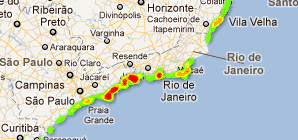
\includegraphics{images/einfuehrung/gmap_fusiontableslayer_heatmap}
	\caption{Daten als Heatmap mit FusionTablesLayer}
	\label{fusiontableslayer-heatmap}
\end{figure}

Leider sind momentan die Konfigurationsmöglichkeiten der Heatmap auf ein Minimum beschränkt. Es ist lediglich möglich zu definieren, ob die Heatmap angezeigt werden soll oder nicht. Eine Legende lässt sich beispielsweise nicht anzeigen. So kann man nicht genau sagen, welche werte nun hinter der grünen oder der roten Farbe stecken. Zudem lassen sich diese Farben auch nicht anpassen.

\subsection{Performance}
Der grösste Vorteil der Fusion Table-Ebenen steckt aber nicht zwingend in den sichtbaren Features. Man findet ihn wohl eher darin, dass die Geocodierungen der Standort-Daten direkt aus der Tabelle gelesen werden und nicht manuell vom Client abgefragt werden müssen. Dadurch kann die Ebene komplett auf den Servern von Google aufbereitet werden. Der Client muss die erhaltenen Daten lediglich noch darstellen. Der Vorteil davon wird durch das folgende Diagramm \ref{fusiontableslayer-compare_markers}\footnote{Quelle: \url{http://www.google.com/events/io/2011/sessions/managing-and-visualizing-your-geospatial-data-with-fusion-tables.html} (Stand: 17.05.2012)} schnell ersichtlich.

\begin{figure}[!h]
	\centering
	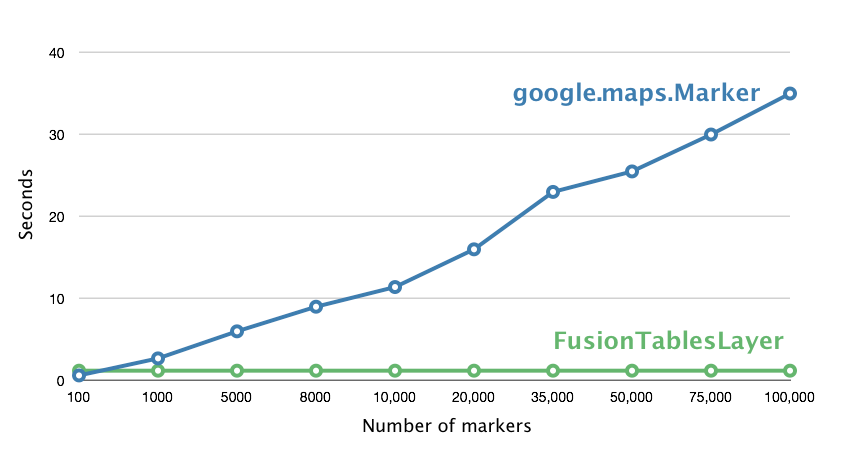
\includegraphics[width=0.9\textwidth]{images/einfuehrung/gmap_fusiontableslayer_vs_markers}
	\caption{FusionTablesLayer verglichen mit Markers}
	\label{fusiontableslayer-compare_markers}
\end{figure}

Die Zeit für das Rendering der Karte bleibt demnach bei der Verwendung von Fusion Table-Ebenen konstant und somit unabhängig von der Anzahl Markierungen, welche gesetzt werden müssen. Der Rechenaufwand, der für das Erstellen der Javascript Marker-Objekte verwendet werden müsste, wird direkt von den Google Servern übernommen und das Resultat als Bild zum Client gesendet. Daraus resultiert die konstante Zeit, welche für die Anfrage zum Server und für das Senden der Antwort zum Client verwendet wird.

\subsection{Einschränkungen}
\subsubsection{Freigabe der Tabelle}
Ein grosser Nachteil der Fusion Table-Ebenen besteht aber darin, dass die verwendeten Fusion Tables als  \emph{öffentlich} markiert sein müssen, um diese auf einer Karte darzustellen. Sprich jeder kann die Tabellen anzeigen oder auslesen. Es ist also nicht möglich eine Tabelle mit sensiblen Daten als Fusion Table-Ebene darzustellen.

Von Google wird zur Lösung dieses Problems aber folgendes Vorgehen vorgeschlagen: Man kann für Tabellen mit sensiblen Inhalten eine View erstellen, welche lediglich die öffentlichen Spalten und Zeilen selektiert. Diese View könnte man dann als \emph{öffentlich} markieren und in einer Fusion Table-Ebene verwenden.

Eine Ausnahme dieser Regelung bilden dabei die Maps API Premier Kunden. Diese haben die Möglichkeit eine Fusion Table als \emph{Protectet Map Layer} freizugeben, wodurch sich diese nur in einer definierten Applikation als Ebene einbinden lässt. Die Datenbank bleibt dabei komplett privat und kann nicht ausgelesen werden.

Die Lizenzpreise für Maps API Premier Kunden beginnen bei 10'000\$ pro Jahr und unterscheiden sich je nach Bedürfnis und Verwendung. 

\subsubsection{Event-Handling auf Fusion Table-Ebenen}
Bislang ist es erst möglich den Klick-Event auf einer Fusion Table-Ebene zu Behandeln. Dieser liefert standardmässig das Template des InfoWindows mit, welches mit dem Klick angezeigt wird. Zudem erhält man die Daten der "`angeklickten Zeile"' beziehungsweise die zugehörigen Daten des angeklickten Objekts auf der Karte. Man hat die Möglichkeit dieses Template anzupassen bevor das InfoWindow angezeigt wird.

Weitere Events können auf einer Fusion Table-Ebene aber noch nicht behandelt werden. Es ist also nicht möglich beispielsweise ein Objekt auf der Karte bei einem MouseOver-Event anders einzufärben oder ähnliches.

Diese fehlenden Möglichkeiten wurden schon oft von anderen FusionTables-Benutzern bei den Google-Entwicklern angefordert, welche dies ebenfalls als ein wichtiges Feature sehen, dass noch implementiert werden muss.

Als Übergangslösung findet sich bereits eine Custom Library mit dem Namen \emph{Fusion Tips} (\url{http://gmaps-utility-gis.googlecode.com/svn/trunk/fusiontips/docs/examples.html}). Diese legt über die Fusion Table-Ebene eine weitere transparente Ebene. Auf dieser Ebene kann man alle Events, welche das Google Maps API anbietet behandeln (somit auch den MouseOver-Event). Sobald die Maus über die Position eines Elementes auf der Fusion Table fährt, sendet der Event einen Request über das SQL API an die Fusion Table und holt sich die Informationen zu der entsprechenden Zeile. So ist es möglich ein neues Element mit der gleichen Form aber beispielsweise einer anderen Farbe darüber zu legen.

Für den Benutzer entsteht so der Effekt als würde sich die Farbe des gehoverten Elementes ändern.

Die Libary wird in folgendem Blog-Artikel noch sehr gut erklärt: \url{http://csessig.wordpress.com/2012/02/07/multiple-layers-and-rollover-effects-for-fusion-table-maps/}

\subsubsection{Weitere Einschränkungen}
Zusätzlich sind die allgemeinen Limitationen der Google Fusion Tables (siehe Tabelle \ref{gft-limitations}) zu beachten.
